\chapter{粲重子半轻单举衰变的初步唯象学分析}
\label{sec:charm_baryon_case}
本章的内容基于我们最近的工作\cite{Shao:2025rel}，我们在该工作中基于粲重子半轻单举衰变过程实现了完成了$\Lambda_c^+$重子中重夸克展开非微扰参数的初步拟合估计并完成了相应的Robust性测试，该结果与bag model以及wave function metod的结果存在较大的偏离，未来对该现象的进一步分析研究是必要的。

第\ref{chapter: D_meson_case_fitting}章对D介子半轻单举衰变的唯象学分析进行了系统性的讨论，然而，将同样的策略应用到粲重子，特别是$\Lambda_c^+$面临着独特的实验挑战。
具体地, 在 $e^{+} e^{-} \rightarrow \Lambda_c^{+} \Lambda_c^{-}$过程中，$\Lambda_c^{+}$在多个质心能量点产生，其纵向极化$\alpha_0$存在能量依赖，将影响$\Lambda_c^+$的轨迹角度并进一步影响衰变末态电子的动力学信息，此外，实验测量的谱会收到有限几何接受度和重建效率的影响而发生畸变。 \tb{以上这些因素将导致实验室系中观测到的电子动量谱并非单一boost下的简单变换结果，而是由多种不同运动学情形叠加而成的复杂卷积谱}。在这种情况下，传统的固定 boost 变换方法完全失效，无法将测量谱直接变换到 $\Lambda_c^{+}$静止系以提取末态电子能量矩并进一步约束重夸克展开的非微扰参数。

为应对这一挑战，本章引入一种基于贝叶斯定理的迭代推断（iterative unfolding）方法。该方法将实验室系到静止系的变换视为一个概率逆问题，不依赖任何关于 boost的先验假设，而是通过蒙特卡洛模拟正向折叠（forward folding）与数据驱动的贝叶斯更新相结合的方式，直接重建出最可能的 $\Lambda_c^{+}$静止系电子能谱。\tb{这一方法最大限度地利用了有限统计量下的全部运动学信息，避免了固定 boost 近似或事件丢弃带来的信息损失。}

在成功重建电子能谱并提取其能量矩之后，我们将这些矩作为实验输入，与 HQET在 1 S 质量方案下的理论预言进行全局拟合。理论表达式包含 NNLO 微扰修正和 $1 / m_c^3$幂修正，并充分考虑了 $\Lambda_c^{+}$作为重子所特有的算符结构（例如，由于轻双夸克处于自旋为零的组态，色磁算符 $\mu_G^2$ 和自旋－轨道算符 $\rho_{L S}^3$ 在 $\Lambda_c^{+}$中严格消失）。通过这种数据驱动的方式，我们首次直接从实验测量中提取了 $\Lambda_c^{+}$的 HQET 参数 $\mu_\pi^2\left(\Lambda_c^{+}\right)$和 $\rho_D^3\left(\Lambda_c^{+}\right)$.

本章的结构安排如下：第\ref{sec:exp_spectrum_rebirth}节介绍 BESIII 实验数据，并详细阐述迭代贝叶斯推断方法、蒙特卡洛模拟流程以及低动量区的理论拟合外推; 
第\ref{sec: error_ana}节 讨论重建能谱和能矩的误差贡献；第\ref{sec: fitting_on_Lambda_c}节给出电子能量矩的 HQET 理论表达式、全局拟合策略及 HQET 参数提取结果；
第\ref{sec:discussion}节对结果进行简单讨论以及本章小节。

\section{实验数据与电子能谱的重建}\label{sec:exp_spectrum_rebirth}
BESIII合作组在7个不同的质心能量采样了$e^{+} e^{-} \rightarrow \Lambda_c^{+} \Lambda_c^{-}$过程的数据\ct{BESIII:2022cmg}，能量覆盖范围从4.6 $\GeV$到4.7 $\GeV$，整理于表\ref{tab:input_parameters_lambdac_inclusive_sl}, \ref{tab:energy_points_alpha}, \ref{tab:electron_spectrum_bins}中。对于每个能量点，BESIII合作组测量了 $\Lambda_c^{+}$的标记产额 $N_{\rm tag}^{(i)}$和极化信息 $\alpha_i$，这些信息对于后续的电子能谱重建至关重要。

为得到质心系的电子能谱，本节采用了一种迭代贝叶斯推断方法，其流程概括见图\ref{fig:flowchart}。该方法利用蒙特卡洛（MC）模拟，基本思想是 从一个初始猜测出发，通过
蒙特卡洛模拟正向折叠（folding）生成实验室系预测谱，与实验数据比较后利用贝叶斯
公式反向更新真值分布，迭代直至收敛。直接反演这一关系是一个典型的病态逆问题\footnote{这一套方法的最大的 motivation在于实验上给的电子能谱是复合谱，是七个能量点叠数据叠加之后的谱。因此不能基于某些naive的假设， triival的对其进行 boost。对应的解决办法是按照inverse problem的思路，利用贝叶斯的方式，基于质心系的假设谱出发，结合七个能量点的权重，去boost到实验室系，然后与真实的实验室系的电子能谱进行比较，产生效率和迁移矩阵，将效率和迁移矩阵作到实验室系的谱上，得到新一轮的质心系的能谱，进行下一次迭代流程。直到卡方值在 1 附近}（ill-posed inverse problem）。

\begin{figure}[h!]
\centering
\tikzset{every picture/.style={line width=0.75pt}}     
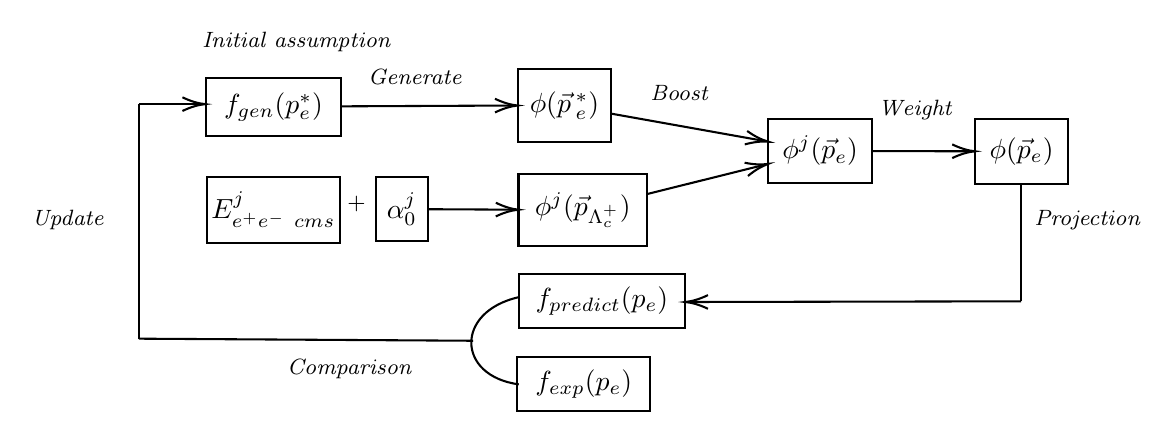
\begin{tikzpicture}[x=0.75pt,y=0.75pt,yscale=-1,xscale=1]

\draw    (290.11,215.67) .. controls (259.11,222.67) and (260.11,253.67) .. (290.11,257.67) ;
\draw    (532.11,217.67) -- (372.33,218) ;
\draw [shift={(370.33,218)}, rotate = 359.88] [color={rgb, 255:red, 0; green, 0; blue, 0 }  ][line width=0.75]    (10.93,-3.29) .. controls (6.95,-1.4) and (3.31,-0.3) .. (0,0) .. controls (3.31,0.3) and (6.95,1.4) .. (10.93,3.29)   ;
\draw    (532.11,161.67) -- (532.11,217.67) ;
\draw    (107.11,235.67) -- (268.11,236.67) ;
\draw    (107.11,122.67) -- (107.11,235.67) ;
\draw    (107.11,122.67) -- (137,122.67) ;
\draw [shift={(139,122.67)}, rotate = 180] [color={rgb, 255:red, 0; green, 0; blue, 0 }  ][line width=0.75]    (10.93,-3.29) .. controls (6.95,-1.4) and (3.31,-0.3) .. (0,0) .. controls (3.31,0.3) and (6.95,1.4) .. (10.93,3.29)   ;

\draw (54,172.33) node [anchor=north west][inner sep=0.75pt]  [font=\footnotesize] [align=left] {\textit{Update}};
\draw (537,172.33) node [anchor=north west][inner sep=0.75pt]  [font=\footnotesize] [align=left] {\textit{Projection}};
\draw (177,244.33) node [anchor=north west][inner sep=0.75pt]  [font=\footnotesize] [align=left] {\textit{Comparison}};
\draw (462,119.33) node [anchor=north west][inner sep=0.75pt]  [font=\footnotesize] [align=left] {\textit{Weight}};
\draw (352,112.33) node [anchor=north west][inner sep=0.75pt]  [font=\footnotesize] [align=left] {\textit{Boost}};
\draw (216,104.33) node [anchor=north west][inner sep=0.75pt]  [font=\footnotesize] [align=left] {\textit{Generate}};
\draw (136,86.33) node [anchor=north west][inner sep=0.75pt]  [font=\footnotesize] [align=left] {\textit{Initial assumption}};
\draw (206,165.33) node [anchor=north west][inner sep=0.75pt]  [font=\footnotesize] [align=left] {+};
\draw    (290.16,204.4) -- (370.16,204.4) -- (370.16,230.4) -- (290.16,230.4) -- cycle  ;
\draw (330.16,217.4) node    {$f_{predict} (p_{e} )$};
\draw    (289.46,244.4) -- (353.46,244.4) -- (353.46,270.4) -- (289.46,270.4) -- cycle  ;
\draw (321.46,257.4) node    {$f_{exp} (p_{e} )$};
\draw    (509.89,129.94) -- (554.89,129.94) -- (554.89,160.94) -- (509.89,160.94) -- cycle  ;
\draw (532.39,145.44) node    {$\phi (\vec{p}_{e} )$};
\draw    (221.28,157.72) -- (246.28,157.72) -- (246.28,188.72) -- (221.28,188.72) -- cycle  ;
\draw (233.78,173.22) node    {$\alpha _{0}^{j}$};
\draw    (139.88,157.66) -- (203.88,157.66) -- (203.88,189.66) -- (139.88,189.66) -- cycle  ;
\draw (171.88,173.66) node    {$E_{e^{+} e^{-} \ cms}^{j}$};
\draw    (289.98,156.2) -- (351.98,156.2) -- (351.98,191.2) -- (289.98,191.2) -- cycle  ;
\draw (320.98,173.7) node    {$\phi ^{j} (\vec{p}_{\Lambda _{c}^{+}} )$};
\draw    (410.33,129.72) -- (460.33,129.72) -- (460.33,160.72) -- (410.33,160.72) -- cycle  ;
\draw (435.33,145.22) node    {$\phi ^{j} (\vec{p}_{e} )$};
\draw    (289.59,105.72) -- (334.59,105.72) -- (334.59,140.72) -- (289.59,140.72) -- cycle  ;
\draw (312.09,123.22) node    {$\phi (\vec{p}\,^{*}_{e})$};
\draw    (139.44,109.88) -- (204.44,109.88) -- (204.44,137.88) -- (139.44,137.88) -- cycle  ;
\draw (171.94,123.88) node    {$f_{gen} (p_{e}^{*} )$};
\draw    (460.33,145.28) -- (507.89,145.39) ;
\draw [shift={(509.89,145.39)}, rotate = 180.13] [color={rgb, 255:red, 0; green, 0; blue, 0 }  ][line width=0.75]    (10.93,-3.29) .. controls (6.95,-1.4) and (3.31,-0.3) .. (0,0) .. controls (3.31,0.3) and (6.95,1.4) .. (10.93,3.29)   ;
\draw    (246.28,173.29) -- (287.98,173.52) ;
\draw [shift={(289.98,173.53)}, rotate = 180.31] [color={rgb, 255:red, 0; green, 0; blue, 0 }  ][line width=0.75]    (10.93,-3.29) .. controls (6.95,-1.4) and (3.31,-0.3) .. (0,0) .. controls (3.31,0.3) and (6.95,1.4) .. (10.93,3.29)   ;
\draw    (351.98,165.98) -- (408.39,151.93) ;
\draw [shift={(410.33,151.45)}, rotate = 166.02] [color={rgb, 255:red, 0; green, 0; blue, 0 }  ][line width=0.75]    (10.93,-3.29) .. controls (6.95,-1.4) and (3.31,-0.3) .. (0,0) .. controls (3.31,0.3) and (6.95,1.4) .. (10.93,3.29)   ;
\draw    (334.59,127.24) -- (408.36,140.41) ;
\draw [shift={(410.33,140.76)}, rotate = 190.12] [color={rgb, 255:red, 0; green, 0; blue, 0 }  ][line width=0.75]    (10.93,-3.29) .. controls (6.95,-1.4) and (3.31,-0.3) .. (0,0) .. controls (3.31,0.3) and (6.95,1.4) .. (10.93,3.29)   ;
\draw    (204.44,123.73) -- (287.59,123.34) ;
\draw [shift={(289.59,123.33)}, rotate = 179.73] [color={rgb, 255:red, 0; green, 0; blue, 0 }  ][line width=0.75]    (10.93,-3.29) .. controls (6.95,-1.4) and (3.31,-0.3) .. (0,0) .. controls (3.31,0.3) and (6.95,1.4) .. (10.93,3.29)   ;

\end{tikzpicture}
\caption{迭代贝叶斯推断方法的流程图：该过程从对 $\Lambda_c^+$ 静止系中电子动量概率密度函数（PDF）的一个任意假设出发，通过将所得模拟的实验室系 PDF 与实验数据进行比较，不断修正这一假设。这里，$f$ 表示电子动量的一维归一化 PDF，而 $\phi$ 表示三维动量矢量空间中的 PDF。$p$ 和 $\vec{p}$ 表示实验室系中的变量，而 $p^*$ 和 $\vec{p}\,^*$ 表示 $\Lambda_c^+$ 静止系中的变量。}
\label{fig:flowchart}
\end{figure}
如图\ref{fig:flowchart}所示，在每一轮迭代中，生成了$10^6$个蒙特卡洛事件，单个事件的生成步骤包括以下几个环节：
\begin{itemize}
    \item \tb{能量点采样:} 根据各能量点的单标记产额 $N_{\mathrm{tag}}$ 构造累积概率分布，按权重随机抽取一个能量点索引 $j$ 。这一步骤确保了 MC 中各能量点的混合比例与真实数据一致。
    \item \textbf{$\Lcp$ 四动量的产生（实验室系）：} 在 $e^{+} e^{-}$质心系中，$\Lambda_c^{+}$的动量模由两体运动学固定：
\begin{equation}
    p_{\mathrm{CMS}}=\frac{\sqrt{s}}{2} \sqrt{1-\frac{4 m_{\Lambda_c}^2}{s}}
\end{equation}
其方向按能量依赖的角分布 $1+\alpha_0(\sqrt{s}) \cos ^2 \theta$ 抽取。为模拟实验室系与质心系之间的微小相对运动，对 $e^{+} e^{-}$系统施加一个沿 $x$ 方向的横向 boost（约 $1.1 \%$ ），再将 $\Lambda_c^{+}$四动量 boost 到实验室系。
    \item \textbf{电子动量抽样}：在 $\Lambda_c^+$ 静止系中，按当前先验分布 $f_{\rm gen}^{(k)}(p_e^*)$ 抽取电子动量模 $p_e^*$（采用 ROOT 的 `TH1::GetRandom()` 方法，按直方图内容加权），并假设衰变末态的电子动量的角度分布各向同性，随机赋予方向。

    \item \textbf{洛伦兹变换到实验室系}：利用 $\Lambda_c^+$ 的四速度 boost 向量 $\boldsymbol{\beta} = \vec{p}_{\Lambda_c}/E_{\Lambda_c}$，将电子四动量从 $\Lambda_c^+$ 静止系 boost 到实验室系。

    \item \textbf{几何接受度约束}：对实验室系中的电子施加极角切割 $|\cos\theta_{\rm lab}| < 0.93$，以模拟 BESIII 探测器的几何接收边界。未通过切割的事件被丢弃。

    \item \textbf{填充直方图与迁移矩阵}：将通过所有步骤的事件按其实验室系动量 $p_e^{\rm lab}$ 填入预测谱 $f_{\rm predict}$，并按 $(p_e^*, p_e^{\rm lab})$ 二维坐标填入迁移矩阵 $\mathcal{M}$。
\end{itemize}
该流程将产生一个基于当前假设的电子动量分布 $f_{predict}(p_e)$与相应的迁移矩阵$\mathcal{M}$,后者表述了$\Lambda_c^+$质心系中生成的电子动量与实验室系中观测到的动量之间的关系。通过比较 $f_{predict}(p_e)$与实验数据 $f_{exp}(p_e)$，并基于贝叶斯定理~\cite{DAgostini:2010hil}更新对 $f_{gen}(p^*_e)$ 的假设，并迭代这一过程直至收敛。

在第k次贝叶斯迭代过程中，有以下的步骤，
\begin{itemize}
        \item \textbf{正向折叠（Folding）}：基于当前先验 $f_{\rm gen}^{(k)}(p_e^*)$，基于上面的MC流程，生成大量蒙特卡洛事件，填充预测实验室系谱 $f_{\rm predict}^{(k)}(p_e^{\rm lab})$ 以及二维迁移矩阵 $\mathcal{M}^{(k)}$。矩阵元 $\mathcal{M}^{(k)}_{ij}$ 定义为：在第 $i$ 个真值分箱中生成、在第 $j$ 个实验室系分箱中观测到的事件数。物理上，这编码了条件概率
    \begin{equation}\label{eq:migration_prob}
        P\bigl(p_e^{\rm lab} \in j \,\big|\, p_e^* \in i\bigr) \propto \mathcal{M}_{ij}^{(k)} .
    \end{equation}

    \item \textbf{效率计算}：对于每个真值分箱 $i$，定义探测效率
    \begin{equation}\label{eq:efficiency}
        \varepsilon_i^{(k)} = \frac{\sum_j \mathcal{M}_{ji}^{(k)}}{N_{\rm gen},i^{(k)}} ,
    \end{equation}
    其中 $N_{\rm gen},i^{(k)}$ 为在第 $i$ 个真值分箱中生成的总事件数。

    \item \textbf{贝叶斯更新}：利用贝叶斯公式，估计实验室系第 $j$ 个分箱中的电子来源于真值第 $i$ 个分箱的概率
    \begin{equation}\label{eq:bayes_prob}
        P^{(k)}(i|j) = \frac{\mathcal{M}_{ij}^{(k)}}{\sum_i \mathcal{M}_{ij}^{(k)}} .
    \end{equation}

    \item \textbf{更新先验}：新的真值分布为
    \begin{equation}\label{eq:update_formula}
        f_{\rm gen}^{(k+1)}(p_e^* \in i) = \frac{1}{\varepsilon_i^{(k)}} \sum_j f_{\rm exp}(p_e^{\rm lab} \in j) \cdot P^{(k)}(i|j) .
    \end{equation}
    该式将实验数据按概率权重分配回真值空间，并以效率进行归一修正。
\end{itemize}
此迭代框架等价于 D'Agostini 方法在存在非均匀 boost 和能量依赖极化情形下的推广。理论上，迭代贝叶斯方法对合理范围内的初始先验不敏感。为验证这一点，本文在系统误差分析中测试了三种不同的初始假设：平坦分布（flat）、多项式函数（polynomial）以及正弦函数（sine）。 nominal 分析采用平坦先验，即将总事件数均匀地分配到 $\Lambda_c^+$ 静止系的各个动量分箱中。

将上述 MC 生成-贝叶斯更新流程迭代执行。每轮迭代结束后，计算预测谱与实验数据的卡方值：
\begin{equation}
    \chi^2/\text{n.d.f.} = \frac{1}{N_{\rm bins}} \sum_{i=1}^{N_{\rm bins}} \frac{\bigl[f_{\rm predict}(p_i) - f_{\rm exp}(p_i)\bigr]^2}{\sigma_i^2} .
\end{equation}
为客观确定最佳迭代次数，本文利用自动扫描机制
\begin{center}
    \texttt{runSingleAnalysis\_autoIter}
\end{center}


在最多 6 轮迭代范围内，选取使 $\chi^2/\text{n.d.f.}$ 最接近 $1$ 的迭代次数作为最优解。扫描结果表明，$k=4$ 轮时 $\chi^2/\text{n.d.f.} = 0.74$，最接近 $1$；继续增加迭代次数时拟合优度不再显著改善，且高阶矩结果在统计涨落范围内保持稳定。因此 nominal 分析取 $N_{\rm iter} = 4$。

图~\ref{fig:result_pe} 展示了unfolding结果：(a) 实验室系中预测谱与实验数据的比较；(b) 从平坦初始猜测经 4 轮迭代后得到的 $\Lambda_c^+$ 静止系电子动量分布。迁移矩阵（图~\ref{fig:result_pe_migration}）清晰显示，在高动量区域存在显著的非对角元，表明单一真值分箱可展宽到较宽的实验室系动量范围。

\begin{figure}[htbp]
    \centering
    \subfloat[模拟得到的实验室系 $p_e$ 概率密度函数（PDF）与测量结果的比较，其中 \(\chindf = 0.74\)。.\label{fig:result_pe_comparison}]{
        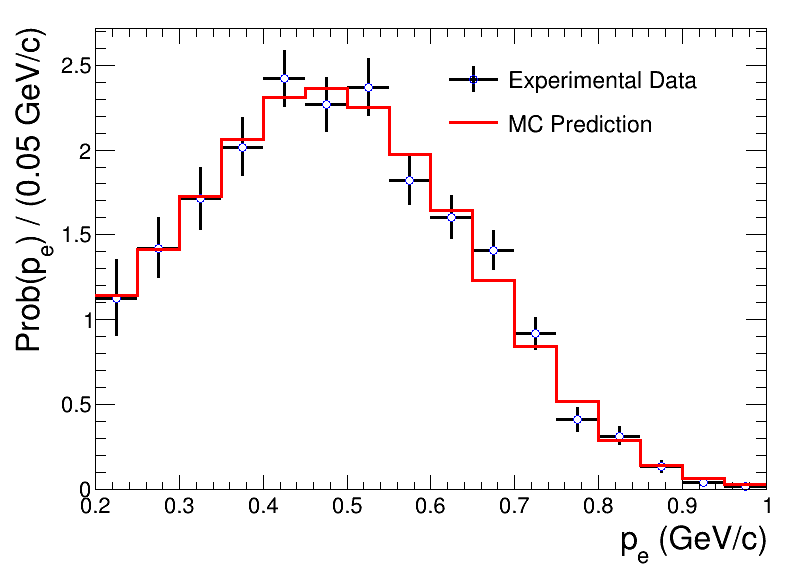
\includegraphics[width=0.48\textwidth]{figures/Lambda_C/data/p_e_comparison.png}
    }
    \hfill
    \subfloat[以平坦分布作为初始假设时，通过贝叶斯推断得到的 \(\Lcp\) 静止系中 $p^*_e$ 的概率密度函数（PDF）。\label{fig:result_pe_Lcrest}]{
        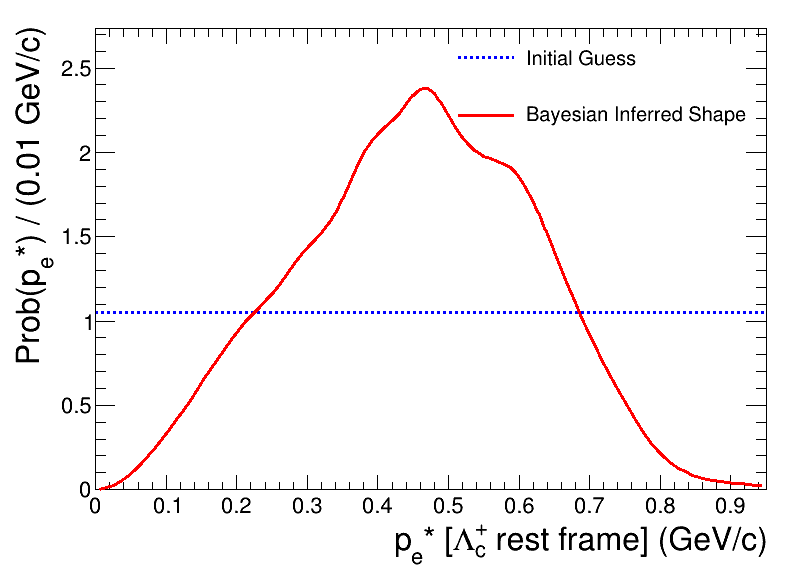
\includegraphics[width=0.48\textwidth]{figures/Lambda_C/data/p_e_Lcrest.png}
    }
    \caption{ $\LcptoXenu$过程质心系电子能谱的重建结果}
    \label{fig:result_pe}
\end{figure}

值得注意的是，实验数据在 $p_e^{\rm lab} < 0.2~\GeV$ 区域因探测器几何边界和重建效率问题而完全缺失。若不作任何处理，Unfolding 过程会在低动量端引入不可控的外推偏差。为此，我们引入一个 HQE 启发的低动量约束。

在远离端点（endpoint）的区域，重夸克展开对半轻单举衰变的电子能谱理论预言的行为良好，可用低阶多项式近似。我们采用如下函数形式：
\begin{equation}\label{eq:low_p_form}
    f(p_e^*) \propto (p_e^*)^2 \bigl(1 + b\, p_e^*\bigr) \bigl(1 - p_e^*\bigr) , \qquad p_e^* < p_{\rm cut} = 0.2~\GeV ,
\end{equation}
其中 $b$ 为自由参数。 具体实现上，在每一轮贝叶斯更新后，我们用式\ref{eq:low_p_form}拟合已展开谱在 $p_e^* \in[0.2,0.4] \mathrm{GeV}$区间的行为，确定参数 $b$ 。随后在 $p_e^*<0.2 \mathrm{GeV} / c$ 区域用该函数进行外推。为保证拼接处的光滑性，要求函数值和一阶导数在 $p_e^*=0.2 \mathrm{GeV}$ 处连续。
\section{谱矩的误差分析：}\label{sec: error_ana}
基于上节最终收敛的$\Lambda_c^+$静止系电子动量分布，我们计算了前四阶归一化能量中心矩 $\langle E_{e,center}^n \rangle$（$n=1,2,3,4$）。本节对谱和能矩的误差进行讨论，误差分为统计误差（由输入数据的有限统计量导致）和系统误差（由分析方法假设和实验输入参数的不确定性导致）。两种误差均用协方差矩阵描述，以便在后续全局拟合中正确处理各矩之间的关联。
\subsection{统计误差：Bootstrap 方法}\label{sec:bootstrap}
统计误差通过 Bootstrap估计。其核心思想是利用原始数据的统计涨落生成大量伪实验样本（toy samples），对每一组样本重复完整的 Unfolding-矩提取流程，最终由结果分布的离散程度确定误差。具体步骤如下：
\begin{itemize}
        \item \textbf{生成Toy samples}：对原始实验谱的每个分箱 $i$，按以中心值 $N_i$ 和误差 $\sigma_i$ 为参数的高斯分布抽取一个波动值 $N_i^{\rm toy}$，得到一组玩具实验谱。共生成 $N_{\rm toys} = 10\,000$ 组独立样本。
    \item \textbf{完整 Unfolding}：对每一组玩具谱，执行与 nominal 分析完全相同的 4 轮贝叶斯迭代 Unfolding，包括相同的 MC 统计量（$10^6$ 事件/轮）和低动量理论约束。
    \item \textbf{提取矩}：从每个展开后的能谱计算四个中心矩 $\langle E_e \rangle$, $M_2$, $M_3$, $M_4$。

    \item \textbf{误差估计}：对每一阶矩，其统计误差取为该矩在 10\,000 个玩具实验上的均方根（RMS）：
    \begin{equation}
        \sigma_{\rm stat}(M_n) = \sqrt{ \frac{1}{N_{\rm toys}} \sum_{t=1}^{N_{\rm toys}} \bigl(M_n^{(t)} - \bar{M}_n\bigr)^2 } ,
    \end{equation}
    其中 $\bar{M}_n$ 为玩具样本上的平均值。
    \item \textbf{协方差矩阵}：四个矩之间的统计关联由 $4\times4$ 样本协方差矩阵描述：
    \begin{equation}
        V_{ij}^{\rm stat} = \frac{1}{N_{\rm toys}-1} \sum_{t=1}^{N_{\rm toys}} \bigl(M_i^{(t)} - \bar{M}_i\bigr) \bigl(M_j^{(t)} - \bar{M}_j\bigr) .
    \end{equation}
\end{itemize}

Bootstrap 给出的统计协方差矩阵列于表~\ref{tab:stat_cov}。可见各矩之间存在一定的负关联，尤其是 $\langle E_e \rangle$ 与 $M_2$ 之间的相关系数约为 $-0.93$，这反映了总能量分布展宽时的补偿效应——若平均能量偏高，则展宽（方差）倾向于减小。

\begin{table}[htbp]
    \centering
    \caption{由 Bootstrap 方法得到的四个电子能量矩的统计协方差矩阵。}
    \label{tab:stat_cov}
    \begin{tabular}{c cccc}
        \toprule
        Stat. Cov. & $\langle E_e\rangle$ [GeV] & $M_2$ [GeV$^2$] & $M_3$ [GeV$^3$] & $M_4$ [GeV$^4$] \\
        \midrule
        $\langle E_e\rangle$ & $2.472\times10^{-4}$ & $-5.315\times10^{-5}$ & $4.762\times10^{-6}$ & $-6.735\times10^{-6}$ \\
        $M_2$ & $-5.315\times10^{-5}$ & $1.314\times10^{-5}$ & $-1.206\times10^{-6}$ & $1.634\times10^{-6}$ \\
        $M_3$ & $4.762\times10^{-6}$ & $-1.206\times10^{-6}$ & $1.926\times10^{-7}$ & $-1.404\times10^{-7}$ \\
        $M_4$ & $-6.735\times10^{-6}$ & $1.634\times10^{-6}$ & $-1.404\times10^{-7}$ & $2.011\times10^{-7}$ \\
        \bottomrule
    \end{tabular}
\end{table}
\subsection{系统误差：Grid Scan 方法}\label{sec:gridscan}
系统误差来源于分析流程中的模型假设和外部输入参数的不确定性。对于基于贝叶斯分迭代实现质心系电子能谱的重建过程中，系统误差的贡献主要有三个来源，本节使用 Grid Scan方法进行讨论。
    \begin{itemize}
        \item \textbf{迭代次数}：贝叶斯迭代的收敛性虽好，但不同迭代次数可能引入微小偏差。我们将 $N_{\rm iter}$ 在 nominal 值 4 的基础上变化为 $\{3, 4, 5\}$。
        \item \textbf{初始先验形状}：虽然方法对合理先验不敏感，但极端形状差异仍可能影响结果。我们测试三种初始假设：平坦分布（nominal）、多项式分布 $1-(2x/p_{\max}-1)^2$、以及正弦分布 $\sin(\pi x/p_{\max})$。
        \item \textbf{极化参数 $\alpha_0$}：$\alpha_0(\sqrt{s})$ 的实验测量存在统计和系统误差。我们将每个能量点的 $\alpha_0$ 整体浮动其总不确定度：$\alpha_0 \to \alpha_0 \pm \sigma_{\alpha_0}^{\rm total}$，其中总误差为统计与系统误差的平方和开根。
    \end{itemize}
上述三个来源共有 $3 \times 3 \times 3 = 27$ 种组合。我们对每一种组合执行完整的 Unfolding-矩提取流程，得到一个四维权空间中的点 $\{\langle E_e \rangle, M_2, M_3, M_4\}$。这组 27 个点构成的集合代表了系统模型假设下的结果变化范围。

系统误差定义为该集合在各矩上的 RMS：
\begin{equation}
    \sigma_{\rm syst}(M_n) = \sqrt{ \frac{1}{27} \sum_{s=1}^{27} \bigl(M_n^{(s)} - \bar{M}_n^{\rm syst}\bigr)^2 } .
\end{equation}
类似地，系统协方差矩阵为：
\begin{equation}
    V_{ij}^{\rm syst} = \frac{1}{27-1} \sum_{s=1}^{27} \bigl(M_i^{(s)} - \bar{M}_i^{\rm syst}\bigr) \bigl(M_j^{(s)} - \bar{M}_j^{\rm syst}\bigr) .
\end{equation}

Grid Scan 的优势在于不需要预先假设各误差源之间的关联结构——27 组结果的联合分布自动编码了所有关联信息\footnote{迭代次数、先验形状和 $\alpha_0$ 的效应在迁移矩阵层面是相互纠缠的。}。

系统协方差矩阵列于表~\ref{tab:syst_cov}。系统误差的大小明显小于统计误差，表明分析结果对方法假设依赖较弱，反映了贝叶斯迭代流程的稳定性。系统关联的模式与统计关联类似，但量级更小。

\begin{table}[htbp]
    \centering
    \caption{由 Grid Scan 方法得到的四个电子能量矩的系统协方差矩阵。}
    \label{tab:syst_cov}
    \begin{tabular}{c cccc}
        \toprule
        Sys. Cov. & $\langle E_e\rangle$ [GeV] & $M_2$ [GeV$^2$] & $M_3$ [GeV$^3$] & $M_4$ [GeV$^4$] \\
        \midrule
        $\langle E_e\rangle$ & $7.031\times10^{-6}$ & $-1.716\times10^{-6}$ & $1.914\times10^{-7}$ & $-1.791\times10^{-7}$ \\
        $M_2$ & $-1.716\times10^{-6}$ & $4.462\times10^{-7}$ & $-3.776\times10^{-8}$ & $4.722\times10^{-8}$ \\
        $M_3$ & $1.914\times10^{-7}$ & $-3.776\times10^{-8}$ & $8.364\times10^{-9}$ & $-1.412\times10^{-9}$ \\
        $M_4$ & $-1.791\times10^{-7}$ & $4.722\times10^{-8}$ & $-1.412\times10^{-9}$ & $6.578\times10^{-9}$ \\
        \bottomrule
    \end{tabular}
\end{table}

表~\ref{tab:final_moments} 给出了四个电子能量矩的最终结果，分别是统计误差和系统误差。

\begin{table}[htbp]
    \centering
    \begin{tabular}{c c}
        \toprule
        能量矩 & 数值 \\
        \midrule
        $\langle E_e \rangle$ [GeV] & $(4.55 \pm 0.16 \pm 0.03) \times 10^{-1}$ \\
        $M_2$ [GeV$^2$] & $(2.75 \pm 0.37 \pm 0.07) \times 10^{-2}$ \\
        $M_3$ [GeV$^3$] & $(-3.67 \pm 4.39 \pm 0.91) \times 10^{-4}$ \\
        $M_4$ [GeV$^4$] & $(1.89 \pm 0.45 \pm 0.08) \times 10^{-3}$ \\
        \bottomrule
    \end{tabular}
        \caption{$\Lambda_c^+ \to X e^+ \nu_e$ 前四阶电子能量中心矩的综合结果。第一个误差为统计，第二个为系统。}
    \label{tab:final_moments}
\end{table}
包含误差的质心系电子能谱与对应的迁移矩阵如图~\ref{fig:exp_finial_results}所示。
\begin{figure}[htbp]
    \centering
    \subfloat[$\LcptoXenu$过程质心系中的电子动量分布unfolded结果 \label{fig:result_pe_final}]{
        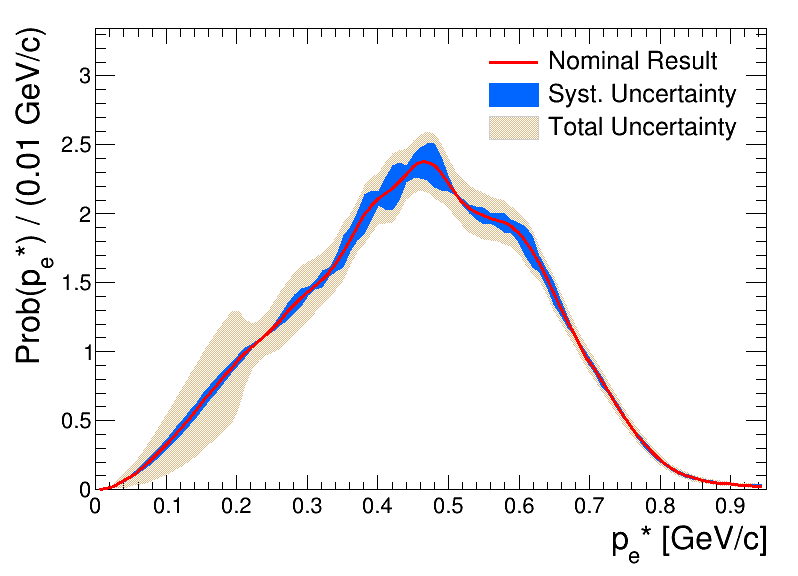
\includegraphics[width=0.48\textwidth]{figures/Lambda_C/data/final_result.png}
    }
    \hfill
    \subfloat[$\Lcp$质心系与实验室系之间电子动量迁移矩阵\label{fig:result_pe_migration}]{
        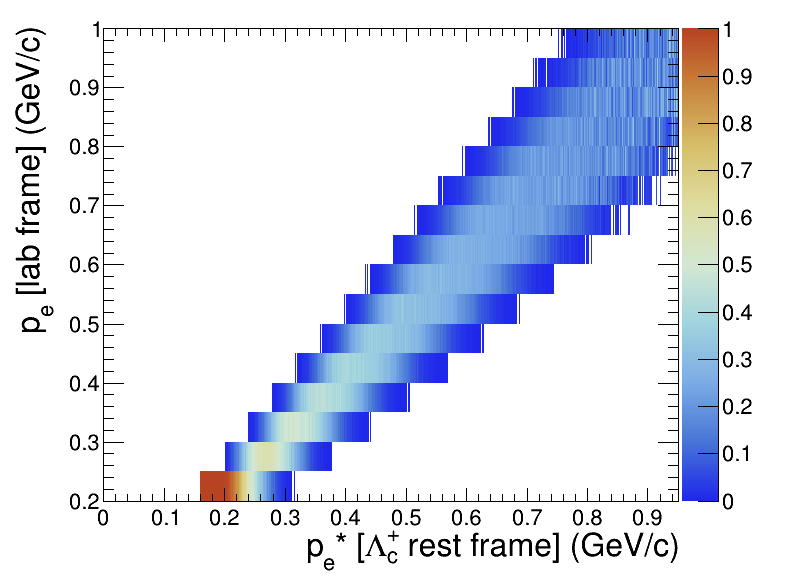
\includegraphics[width=0.48\textwidth]{figures/Lambda_C/data/p_e_migration.png}
    }
    \caption{最终unfolded结果与迁移矩阵}
    \label{fig:exp_finial_results}
\end{figure}
这些矩及其完整的误差协方差信息将作为下一节全局拟合的实验输入，用以约束 $\Lambda_c^+$ 的 HQET 非微扰参数\footnote{考虑到能矩之间的关联效应，实际拟合过程使用衰变宽度、归一化的二、三阶能量中心矩以及四阶中心矩与二阶中心矩平方的比值。尽管物理量存在变化，但其分析流程类似。}。
\section{理论计算结果与重夸克展开非微扰参数的拟合估计}\label{sec: fitting_on_Lambda_c}
\subsubsection{衰变宽度}
不同于粲介子的情形，对于$\Lambda_c^+$，由于ud夸克组成的diquark自旋为0，导致描述重夸克与轻自由度之间色磁相互作用非微扰算符矩阵元$\mu_{G}^2（\Lcp）$和描述轨道-自旋相互作用的非微扰算符矩阵元$\rho_{LS}^3(\Lcp)$的贡献消失。 在极质量方案中，衰变宽度的表达式为
\begin{equation}\label{eq:decay_width}
\begin{aligned}
\Gamma_{\Lambda_c^+} = \sum_{q=d,s} \hat\Gamma_0 |V_{cq}|^2 m_c^5 \Big\{ 1 &+ \frac{\alpha_s}{\pi}\frac{2}{3}\Big(\frac{25}{4}-\pi^2\Big) \\
&+ \frac{\alpha_s^2}{\pi^2}\Big[ \frac{\beta_0}{4}\frac{2}{3}\Big(\frac{25}{4}-\pi^2\Big)\ln\frac{\mu^2}{m_c^2} + 2.14690\,n_l - 29.88311 \Big] \\
& - 8\rho\,\delta_{sq} - \frac{1}{2}\frac{\mu_\pi^2(\Lambda_c^+)}{m_c^2} \\
& + \Big(\frac{20}{3} + 8\ln\frac{\mu^2}{m_c^2}\Big) \frac{\rho_D^3(\Lambda_c^+)}{m_c^3} + \frac{\tau_0(\Lambda_c^+)}{m_c^3} + \cdots \Big\} ,
\end{aligned}
\end{equation}
其中 $\hat\Gamma_0 = G_F^2/(192\pi^3)$，$\rho = m_s^2/m_c^2$，$\beta_0 = 11 - 2n_f/3$（取 $n_f=4$）。$$\tau_{\Lambda_c^{+}}=128 \pi^2\left(T_1\left(\Lambda_c^{+}\right)-T_2\left(\Lambda_c^{+}\right)\right),$$ 代表量纲六算符中四夸克算符矩阵元贡献\cite{Fael:2019umf}。
前四阶电子能量矩的理论表达式同样在极质量方案中给出：
\begin{equation}\label{eq:moment_theory}
\begin{aligned}
\langle E_e\rangle &= \frac{\hat\Gamma_0}{\Gamma_{\Lambda_c^+}} \sum_{q=d,s} |V_{cq}|^2 m_c^6 \Big[ \frac{3}{10} + \frac{\alpha_s}{\pi} a_1^{(1)} + \frac{\alpha_s^2}{\pi^2} a_1^{(2)} - 3\rho\delta_{sq} \\
&\qquad\qquad + \Big(\frac{77}{15} + 4\ln\frac{\mu^2}{m_c^2}\Big)\frac{\rho_D^3}{m_c^3} + \frac{\tau_0}{2m_c^3} + \cdots \Big] , \\
\langle E_e^2\rangle &= \frac{\hat\Gamma_0}{\Gamma_{\Lambda_c^+}} \sum_{q=d,s} |V_{cq}|^2 m_c^7 \Big[ \frac{1}{10} + \frac{\alpha_s}{\pi} a_2^{(1)} + \frac{\alpha_s^2}{\pi^2} a_2^{(2)} - \frac{6}{5}\rho\delta_{sq} + \frac{1}{12}\frac{\mu_\pi^2}{m_c^2} \\
&\qquad\qquad + \Big(\frac{181}{60} + 2\ln\frac{\mu^2}{m_c^2}\Big)\frac{\rho_D^3}{m_c^3} + \frac{\tau_0}{4m_c^3} + \cdots \Big] , \\
\langle E_e^3\rangle &= \frac{\hat\Gamma_0}{\Gamma_{\Lambda_c^+}} \sum_{q=d,s} |V_{cq}|^2 m_c^8 \Big[ \frac{1}{28} + \frac{\alpha_s}{\pi} a_3^{(1)} + \frac{\alpha_s^2}{\pi^2} a_3^{(2)} - \frac{1}{2}\rho\delta_{sq} + \frac{1}{14}\frac{\mu_\pi^2}{m_c^2} \\
&\qquad\qquad + \Big(\frac{233}{140} + \ln\frac{\mu^2}{m_c^2}\Big)\frac{\rho_D^3}{m_c^3} + \frac{\tau_0}{8m_c^3} + \cdots \Big] , \\
\langle E_e^4\rangle &= \frac{\hat\Gamma_0}{\Gamma_{\Lambda_c^+}} \sum_{q=d,s} |V_{cq}|^2 m_c^9 \Big[ \frac{3}{224} + \frac{\alpha_s}{\pi} a_4^{(1)} + \frac{\alpha_s^2}{\pi^2} a_4^{(2)} - \frac{3}{14}\rho\delta_{sq} + \frac{3}{64}\frac{\mu_\pi^2}{m_c^2} \\
&\qquad\qquad + \Big(\frac{1989}{2240} + \frac{1}{2}\ln\frac{\mu^2}{m_c^2}\Big)\frac{\rho_D^3}{m_c^3} + \frac{\tau_0}{16m_c^3} + \cdots \Big] .
\end{aligned}
\end{equation}
其中系数 $a_n^{(1)}$、$a_n^{(2)}$ 为已知的 NLO 和 NNLO 微扰修正\cite{Shao:2025vhe}。上式中的 $\mu_\pi^2$、$\rho_D^3$、$\tau_0$ 均省略了 $(\Lambda_c^+)$ 标记，但默认指 $\Lambda_c^+$ 的矩阵元。

从式~\eqref{eq:decay_width} 和 \eqref{eq:moment_theory} 可以观察到，高阶矩对 $\mu_\pi^2$ 和 $\rho_D^3$ 的敏感度逐渐增强（系数增大），但同时实验测量值的误差也增大，即无法通过无限制地增加矩阶数来获得更精确的非微扰参数约束。实际拟合中，我们选择使用衰变宽度、归一化的平均能量 $\langle E_e \rangle$、归一化的二阶中心矩 $M_2$ 以及四阶中心矩与二阶中心矩平方的比值 $M_4/M_2^2$ 作为输入物理量，以充分利用矩之间的相关性并避免高阶矩过大的统计误差。


基于D介子sector中对非微扰参数的拟合经验，本节在1S质量方案下进行拟合估计。为抑制各矩之间的关联，我们在拟合中使用中心矩而非原始矩。具体地，定义五个观测量：
\begin{equation}
\boldsymbol{y} = \Big\{ \Gamma_{\Lambda_c^+},\; \langle E_e\rangle,\; \langle E_e^2\rangle_c,\; \langle E_e^3\rangle_c,\; \frac{\langle E_e^4\rangle_c}{\langle E_e^2\rangle_c^2} \Big\} .
\end{equation}
其中 $\Gamma_{\Lambda_c^+}$ 为 $\Lambda_c^+$ 的总衰变宽度（取自 PDG），其余四个量来自上一节的 Unfolding 重建结果。将 $\langle E_e^4\rangle_c$ 除以其方差的平方是为了降低高阶矩之间的强关联现象，使各数据点均可被充分利用。


拟合$\chi^2$ 函数定义如下：
\begin{equation}\label{eq:chi2}
\chi^2(\boldsymbol{\theta}) = \bigl[\boldsymbol{y} - \boldsymbol{\eta}(\boldsymbol{\theta})\bigr]^T \boldsymbol{V}^{-1} \bigl[\boldsymbol{y} - \boldsymbol{\eta}(\boldsymbol{\theta})\bigr] ,
\end{equation}
其中 $\boldsymbol{\theta} = \{\mu_\pi^2(\Lambda_c^+),\, \rho_D^3(\Lambda_c^+),\, \tau_{\rm WA}(\Lambda_c^+)\}$ 为待拟合参数。四夸克贡献被参数化为
\begin{equation}
\tau_{\rm WA}(\Lambda_c^+) = |V_{cs}|^2 \tau_{0,\rm non-valence} + |V_{cd}|^2 \tau_{0,\rm valence} .
\end{equation}

权重矩阵 $\boldsymbol{V}$ 取为统计协方差矩阵与系统协方差矩阵之和：$\boldsymbol{V} = \boldsymbol{V}^{\rm stat} + \boldsymbol{V}^{\rm syst}$，即表~\ref{tab:stat_cov} 和表~\ref{tab:syst_cov} 所给出的结果。由于五个观测量中只有后四个来自 Unfolding，衰变宽度的误差与能谱矩的误差之间无关联，因此 $\boldsymbol{V}$ 的 $(1,2\text{--}5)$ 非对角元为零。
为估计理论输入参数引入的误差，本节讨论了重整化能标跑动引入的误差，即理论表达式的标度依赖性。重整化能标$\mu$在区间 $1~\GeV \le \mu \le 2\overline{m}_c(\overline{m}_c) \approx 2.54~\GeV$ 内扫描\footnote{对应于两千次扫描拟合，如图\ref{fig:result_chi2_RGrunning_Lcrest}所示，其有效最小$\chi^2$落在0到2之间，该结果表明尽管重整化能标的部分扫描过于靠近非微扰能标，但基于1S质量方案下的扫描拟合结果仍可接受。}，扫描拟合的中心值浮动作为来自理论输入参数带来的误差贡献。
\section{结果讨论}\label{sec:discussion}
由于待拟合参数过少，本节使用的理论表达式包含两圈图的微扰修正与包含量纲六算符四夸克算符号的幂次修正。为保守估计,本节引入$30\%$的相对误差以反映高阶幂次修正引入的误差。具体地，我们采用代码文件
\begin{center}
    \verb|Fitting_on_Lambda_c.nb/Scenario-3_Reduced|
\end{center}
中case-1（拟合估计中心值）,case-2（估计来自重整化能标$\mu$地跑动引入的误差），case-3（鲁棒性测试）的结果。 为检验固定能标处的拟合稳定性，我们基于实验数据及其误差，采用MC生成500组toy实验数据；基于该500组实验数据完成对应的拟合\footnote{假设toy实验数据之间的误差关联与real实验数据的误差关联保持一致}。观察500组拟合结果的分布，如图\ref{fig:result_Lambda_c_rb}所示，大多数拟合结果均落在固定能标处real数据拟合结果的1倍标准误差内，这表明了固定能标处的拟合估计具有很好的稳定性。全局拟合在 1S 质量方案下给出以下结果（表~\ref{tab:fit_result}）：

\begin{table}[htbp]
    \centering
    \begin{tabular}{l c}
        \toprule
        参数 & 拟合值 \\
        \midrule
        $\mu_\pi^2(\Lambda_c^+)~[10^{-1}~\GeV^2]$ & $1.33 \pm 0.18 \pm 0.02 \pm 0.40$ \\
        $\rho_D^3(\Lambda_c^+)~[10^{-4}~\GeV^3]$ & $-2.95 \pm 2.59 \pm 0.36 \pm 1.18$ \\
        $\tau_{\rm WA}(\Lambda_c^+)~[10^{-1}~\GeV^3]$ & $-2.69 \pm 0.33 \pm 0.12 \pm 0.81$ \\
        \midrule
        $\chi^2/\text{d.o.f.}$ & $0.53$ \\
        数据点数 / 参数数 & $5$ / $3$ \\
        \bottomrule
    \end{tabular}
        \caption{1S 质量方案下的全局拟合结果。三项误差依次为：实验误差、重整化标度误差、高阶幂修正估计误差(中心值的30\%)。}
    \label{tab:fit_result}
\end{table}

拟合参数之间存在非平凡的关联，尤其是 $\mu_\pi^2$ 与 $\rho_D^3$ 之间呈现显著的负关联。图~\ref{fig:result_ellipse_Lcrest} 展示了 $(\mu_\pi^2, \rho_D^3)$ 平面上的 $1\sigma$ 和 $2\sigma$ 误差椭圆。该椭圆由拟合的 Hessian 矩阵在 $(\mu_\pi^2, \rho_D^3)$ 子空间中投影得到。

\begin{figure}[htbp]
    \centering
    \subfloat[$\mu^{2}(\Lcp)-\rho_D^3(\Lcp)$平面误差椭圆，其包含两方面的贡献，分别是包含来自实验数据的误差和重整化能标跑动引入的误差.\label{fig:result_ellipse_Lcrest}]{
        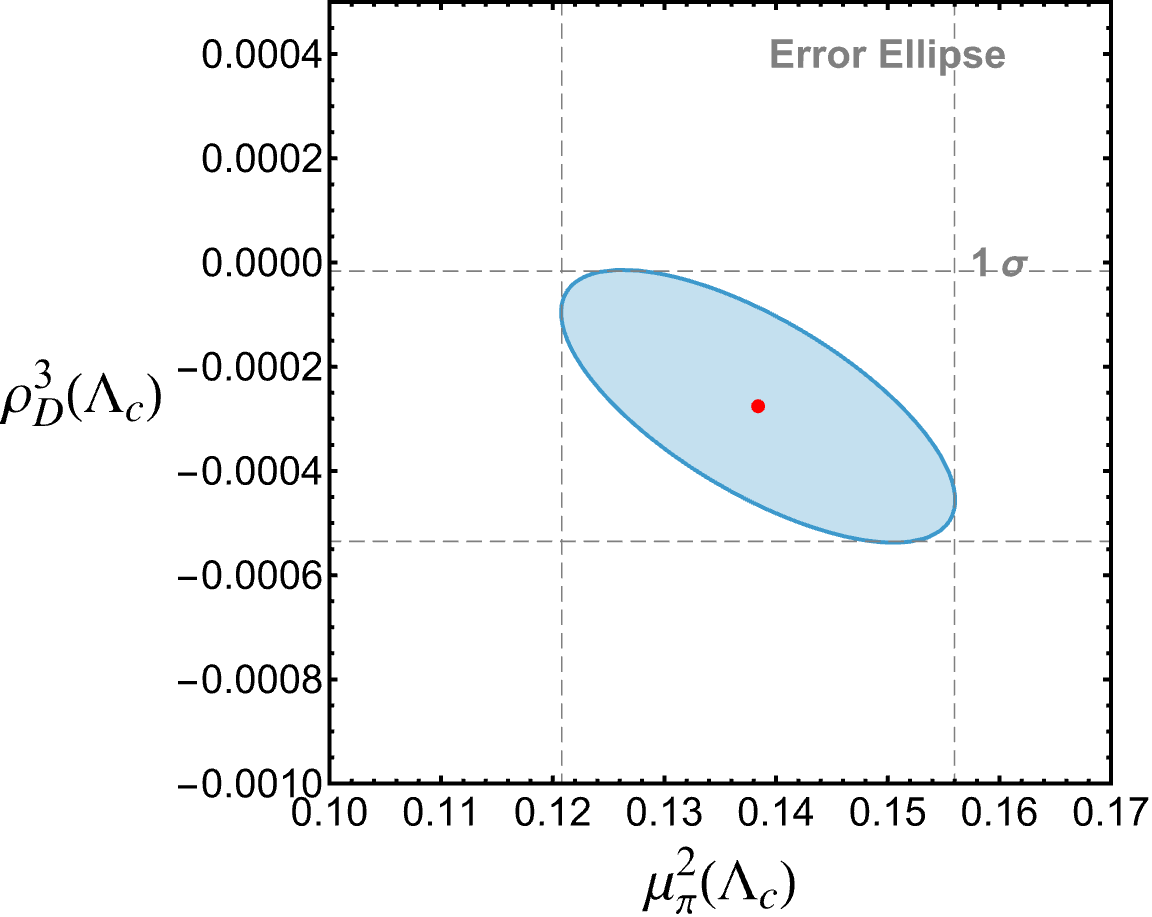
\includegraphics[width=0.48\textwidth]{figures/Lambda_C/Global_Fitting/Error_pllise.png}
    }
    \hfill
    \subfloat[重整化能标跑动情形下对应的拟合结果$\chi^2$分布\label{fig:result_chi2_RGrunning_Lcrest}]{
        \raisebox{0.10\height}{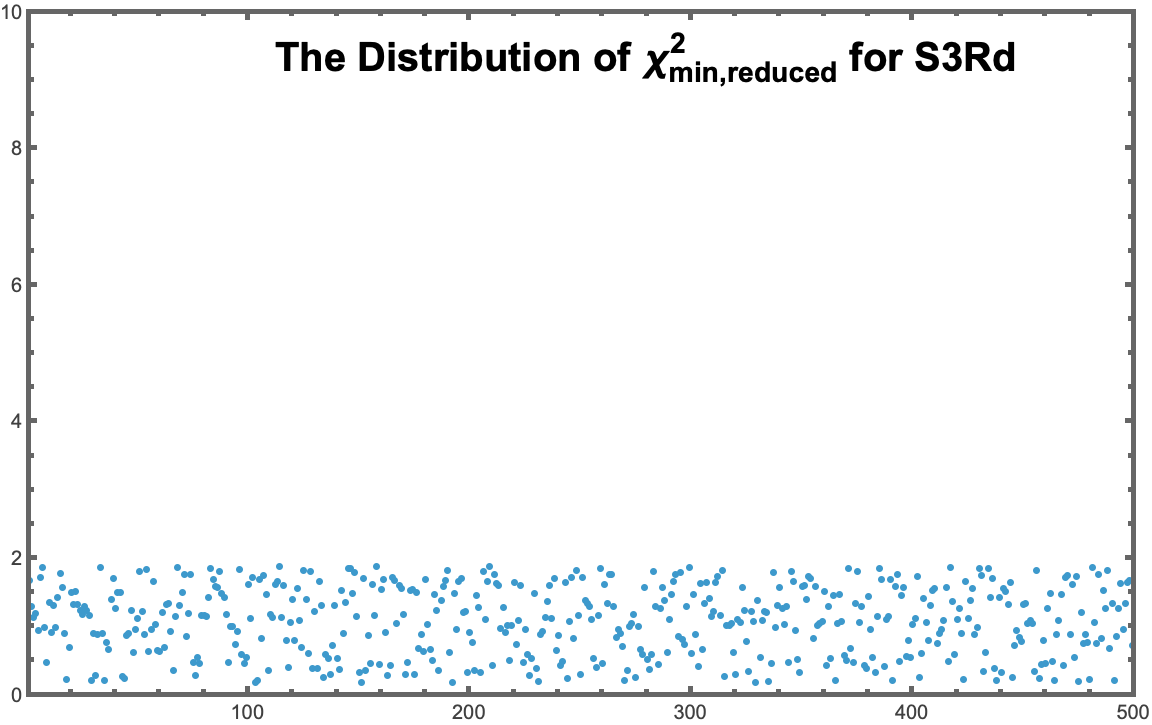
\includegraphics[width=0.48\textwidth]{figures/Lambda_C/Global_Fitting/chi_2_rg.png}}
    }
    \caption{基于$\LcptoXenu$过程的HQE非微扰参数的拟合结果}
    \label{fig:result_Lcrest}
\end{figure}
表~\ref{tab:compare_mesons} 汇总了 1S 质量方案下，$\Lambda_c^+$ 与 $D^0$、$D^+$、$D_s^+$ 的 $\mu_\pi^2$ 和 $\rho_D^3$ 提取结果。

\begin{table}[htbp]
    \centering
    \begin{tabular}{lcc}
        \toprule
        强子 & $\mu_\pi^2~[\GeV^2]$ & $\rho_D^3~[\GeV^3]$ \\
        \midrule
        $D^0$ & $0.15 \pm 0.02$ & $0.03 \pm 0.03$ \\
        $D^+$ & $0.16 \pm 0.02$ & $-0.01 \pm 0.03$ \\
        $D_s^+$ & $0.18 \pm 0.03$ & $-0.02 \pm 0.04$ \\
        $\Lambda_c^+$（本章） & $0.133 \pm 0.018 \pm 0.002 \pm 0.040$ & $-0.000295 \pm 0.000259 \pm 0.000036 \pm 0.000118$ \\
        \bottomrule
    \end{tabular}
        \caption{1S 质量方案下粲强子 HQET 参数的比较}
    \label{tab:compare_mesons}
\end{table}

从表~\ref{tab:compare_mesons} 可见，$\Lambda_c^+$ 的 $\mu_\pi^2$ 与 D 介子的结果在 $1\sigma$ 范围内一致，但中心值略低于 $D^0$ 和 $D^+$。这一趋势在物理上是可预期的：$\Lambda_c^+$ 中的轻双夸克处于自旋为零的组态，其空间波函数与介子中的轻夸克-反夸克对有所不同，导致重夸克在 $\Lambda_c^+$ 内部感受到的有效动能略有差异。

$\rho_D^3$ 的比较则更为微妙。D 介子的 $\rho_D^3$ 中心值接近于零，而 $\Lambda_c^+$ 的结果为负值，但误差较大。考虑到 $\Lambda_c^+$ 的 $\rho_D^3$ 提取首次实现，其不确定度仍显著大于 D 介子情形，这主要源于当前可用的实验输入仅有 5 个数据点。随着未来 BESIII 更多能量点数据或 Belle~II 相关分析的积累，$\rho_D^3(\Lambda_c^+)$ 的精度有望大幅提升。

需要强调的是，$\Lambda_c^+$ 与 D 介子之间最显著的差异并非体现在 $\mu_\pi^2$ 或 $\rho_D^3$ 的数值上，而是体现在 HQE 的算符结构中：在 $\Lambda_c^+$ 中 $\mu_G^2 = \rho_{LS}^3 = 0$，而在 D 介子中这些算符贡献非零。这意味着，即使 $\mu_\pi^2$ 和 $\rho_D^3$ 数值相近，它们对物理可观测量（如衰变宽度、寿命比）的实际影响路径也不同。

\subsection{与模型计算的比较}

除数据驱动提取外，$\Lambda_c^+$ 的 HQET 参数也可通过非微扰模型估算。我们将本章结果与两种主要模型进行对比：

\textbf{（1）改进袋模型（Improved Bag Model）}

Cheng 等人\cite{Cheng:2023jpz}利用改进的相对论袋模型计算了 $\Lambda_c^+$ 的矩参数，得到 $\mu_\pi^2 \approx 0.42~\GeV^2$，$\rho_D^3 \approx 0.02~\GeV^3$显著高于本章的拟合估计值。袋模型的偏差可能来源于其对轻夸克波函数的简化处理——袋模型假设夸克被限制在球形空腔内，而真实强子中的轻双夸克可能具有更复杂的关联结构，对该偏离背后原因的进一步讨论是必要的。

\textbf{（2）波函数方法（Wave-function Approach）}

Gratrex 等人\cite{Gratrex:2022xpm}采用波函数的方法，得到 $\mu_\pi^2 \approx 0.5~\GeV^2$ 和 $\rho_D^3 \approx 0.04~\GeV^3$。波函数方法的结果与本章数据提取结果同样具有较大的偏离，尤其是在 $\mu_\pi^2$ 。这些差异源于模型计算对轻夸克动力学和强子波函数的细节敏感，而不同模型对这些非微扰效应的处理方式各异。相比之下，本章的数据驱动方法避免了模型依赖，直接将理论矩与实验测量关联。随着未来数据点的数量不断增多且实现对非微扰参数的更高精度的拟合分析，对data-driven和模型计算之间的偏离讨论本身是有意义的——它为未来改进非微扰模型提供了思路。

\begin{figure}[htbp]
    \centering

    \subfloat[最小$\chi^2$分布。\label{fig:chi_2_rb_Lcrest}]{
        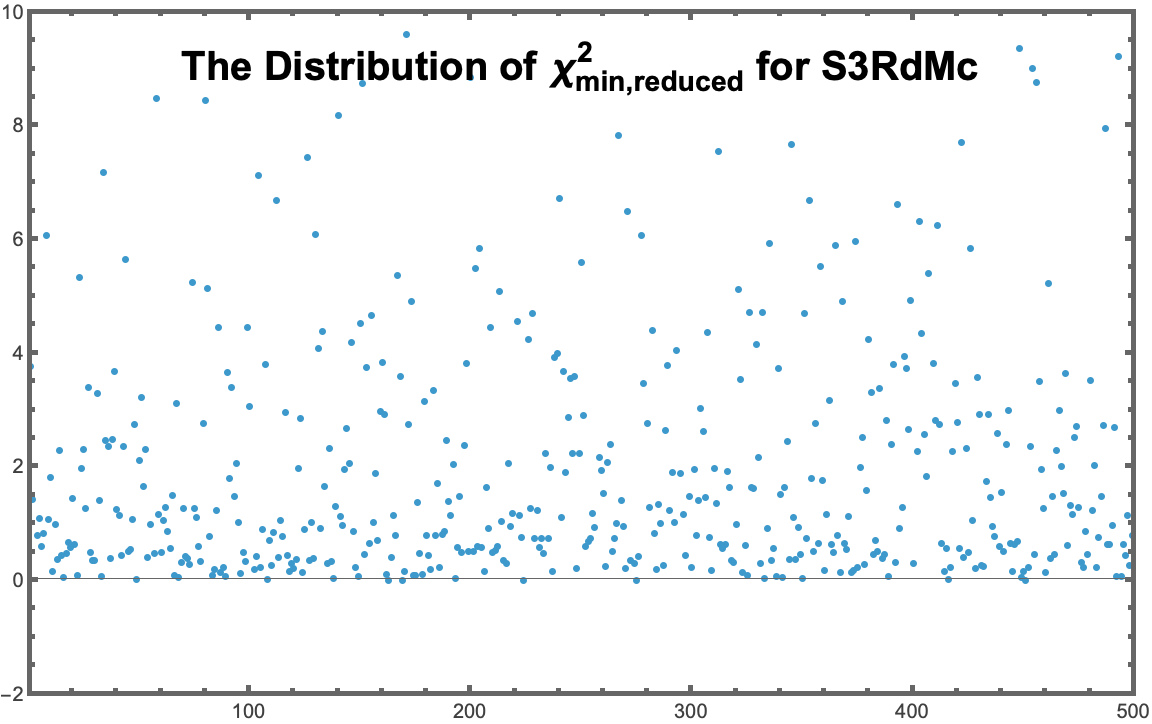
\includegraphics[width=0.48\textwidth]{figures/Lambda_C/Global_Fitting/chi_2_rb.png}
    }
    \hfill
    \subfloat[$\mu_{\pi^2}(\Lcp)$拟合结果分布\label{fig:mupi2_Rb_Lcrest}]{
        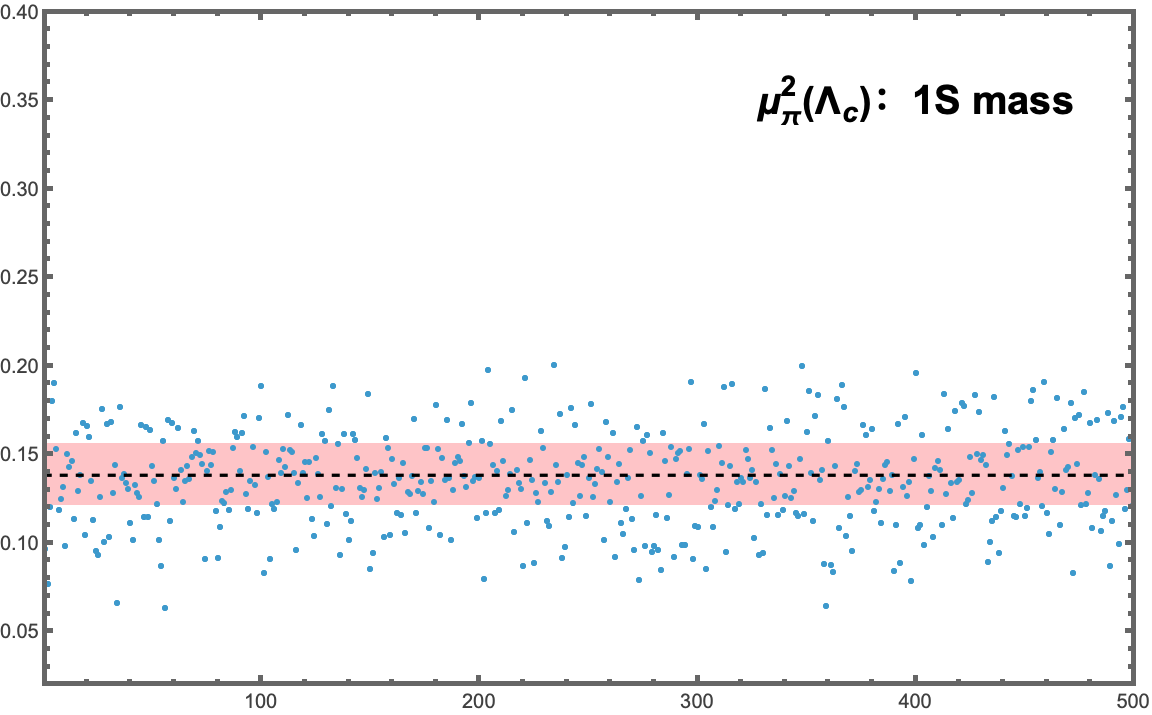
\includegraphics[width=0.48\textwidth]{figures/Lambda_C/Global_Fitting/mupi2_Rb.png}
    }

    \vspace{0.5em}

    \subfloat[$\rho_{D}^3(\Lcp)$拟合结果分布\label{fig:rhoD3_Rb_Lcrest}]{
        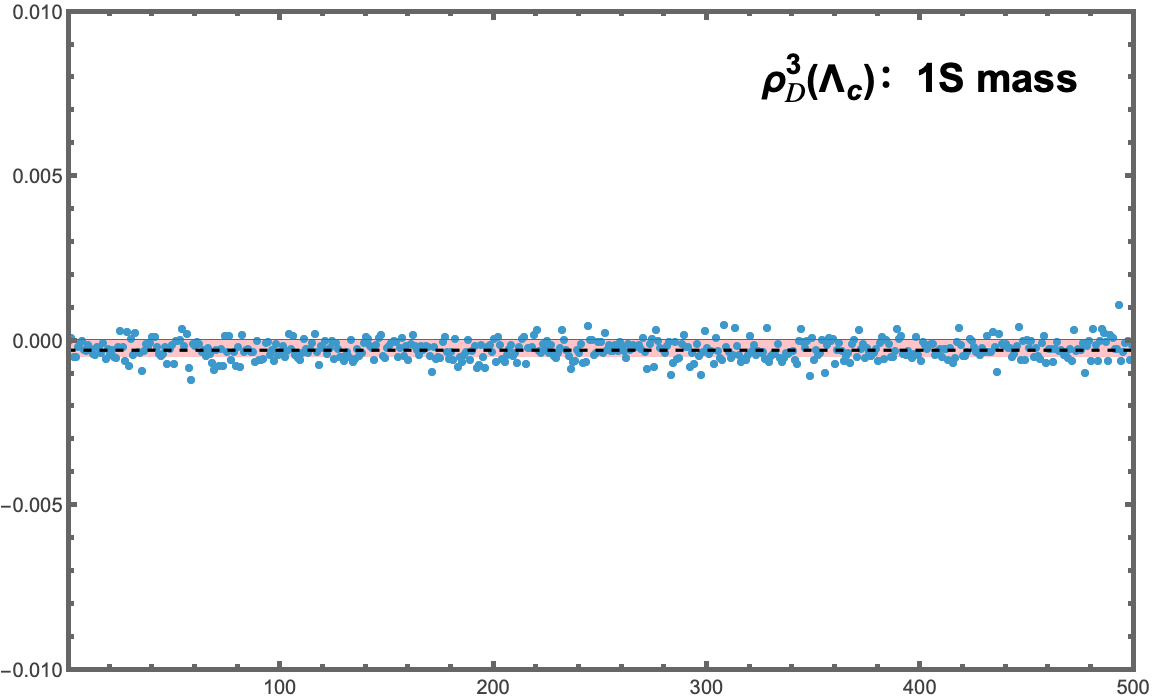
\includegraphics[width=0.48\textwidth]{figures/Lambda_C/Global_Fitting/rhoD3_Rb.png}
    }
    \hfill
    \subfloat[弱湮灭参数的拟合结果分布\label{fig:tauWA_Rb_Lcrest}]{
        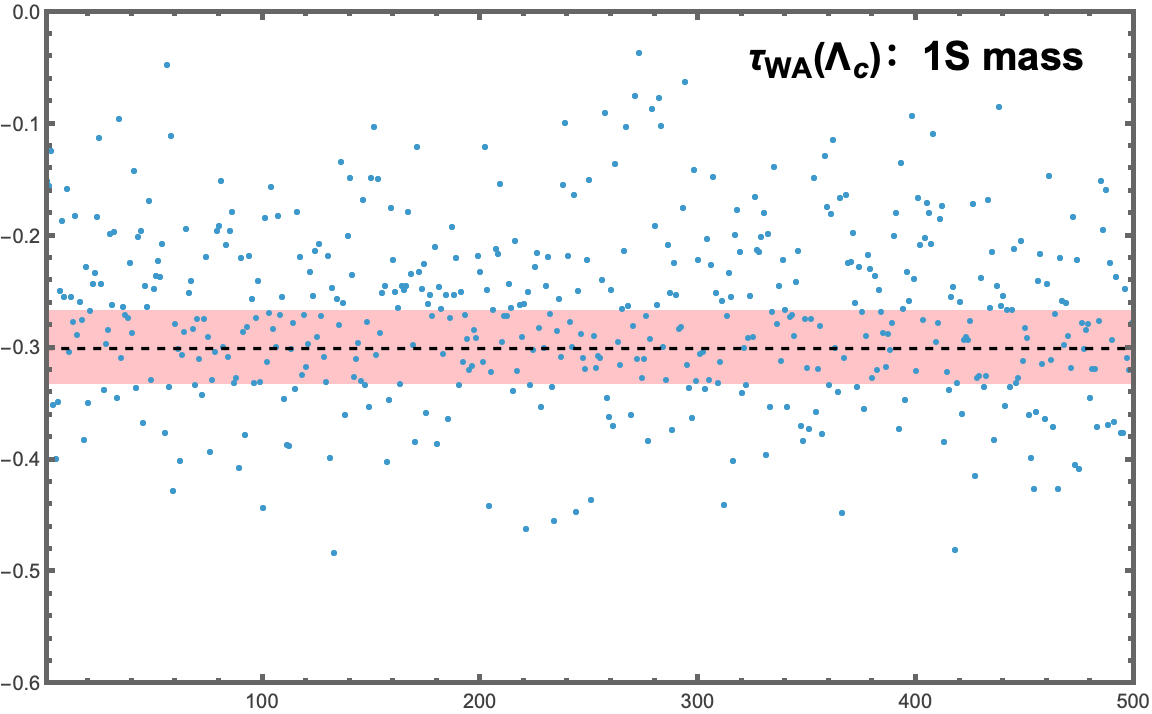
\includegraphics[width=0.48\textwidth]{figures/Lambda_C/Global_Fitting/tauWA_Rb.png}
    }

    \caption{基于500组toy experiment data的拟合结果分布。每个子图展示了对应参数的拟合结果分布，红色参考线表示固定能标处real数据拟合结果的中心值，蓝色误差带表示该中心值的1倍标准误差范围。大多数拟合结果均落在$1-2\sigma$范围内，表明固定能标处的拟合估计具有很好的稳定性。}
    \label{fig:result_Lambda_c_rb}
\end{figure}

\newpage
\section{附：实验数据}
\begin{table}[htbp]
\centering
\renewcommand{\arraystretch}{1.15}
\begin{tabular}{lll}
\hline\hline
\textbf{物理量} & \textbf{数值} & \textbf{内容} \\
\hline
$m_e$ & $0.000510999~\mathrm{GeV}$ & 电子质量 \\
$m_n$ & $0.939565~\mathrm{GeV}$ & 中子质量 \\
$m_{\Lambda_c}$ & $2.28646~\mathrm{GeV}$ & $\Lambda_c^+$ 质量 \\
$n_{\rm energy\ points}$ & $7$ & $\sqrt{s}$ 能量点数 \\
$n_{\rm total\ MC\ events}$ & $10^6$ & 总蒙特卡洛事件数 \\
$n_{\rm bins}^{\rm reco}$ & $16$ & 重构动量分箱数 \\
$\Delta p_{\rm true}$ & $0.01~\mathrm{GeV}/c$ & 真实水平分辨率 \\
$p_{\min}^{\rm lab}$ & $0.2~\mathrm{GeV}/c$ & 实验室系电子最小动量 \\
$p_{\max}^{\rm lab}$ & $1.0~\mathrm{GeV}/c$ & 实验室系电子最大动量 \\
$|\cos\theta|_{\rm track}$ & $<0.93$ & 探测器几何约束 \\
\hline\hline
\end{tabular}
\caption{$\Lambda_c^+ \to X e^+ \nu_e$ 电子能谱重建的输入参数设置。}
\label{tab:input_parameters_lambdac_inclusive_sl}
\end{table}
\begin{table}[htbp]
\centering
\footnotesize
\setlength{\tabcolsep}{4pt}
\renewcommand{\arraystretch}{1.15}
\begin{tabular}{@{}cccc@{}}
\hline\hline
\multicolumn{3}{c}{$\Lambda_c^+$ 标记产额} & $\alpha_i$ 及其误差 \\
\hline
$i$ & $\sqrt{s}_i~(\mathrm{GeV})$ & $N_{\rm tag}^{(i)}$ & $\alpha_i \pm \delta\alpha_i^{\rm stat} \pm \delta\alpha_i^{\rm syst}$ \\
\hline
1 & 4.59953 & 17978 & $-0.20\pm0.04\pm0.02$ \\
2 & 4.61186 & 3357  & $-0.26\pm0.09\pm0.01$ \\
3 & 4.62800 & 13699 & $-0.21\pm0.04\pm0.01$ \\
4 & 4.64091 & 15711 & $-0.09\pm0.05\pm0.01$ \\
5 & 4.66124 & 14895 & $-0.02\pm0.05\pm0.01$ \\
6 & 4.68192 & 44132 & $0.15\pm0.03\pm0.01$ \\
7 & 4.69882 & 12693 & $0.34\pm0.07\pm0.01$ \\
\hline\hline
\end{tabular}
\caption{BESIII合作组在不同质心能量点测量的 $\Lambda_c^+$ 标记产额与极化信息，$\alpha_i$ 及其统计/系统误差以 $\pm$ 形式给出}
\label{tab:energy_points_alpha}
\end{table}
\begin{table}[htbp]
\centering
\renewcommand{\arraystretch}{1.15}
\begin{tabular}{cccccccc}
\hline\hline
\textbf{Bin} & $p_e^{\rm lab}$ range $(\mathrm{GeV}/c)$ & $N_e$ & $\delta N_e$&\textbf{Bin} & $p_e^{\rm lab}$ range $(\mathrm{GeV}/c)$ & $N_e$ & $\delta N_e$ \\
\hline
1  & $[0.20,\,0.25)$ & 244 & 49 &9  & $[0.60,\,0.65)$ & 347 & 28 \\
2  & $[0.25,\,0.30)$ & 308 & 39 &10 & $[0.65,\,0.70)$ & 305 & 26 \\
3  & $[0.30,\,0.35)$ & 371 & 40 &11 & $[0.70,\,0.75)$ & 199 & 21 \\
4  & $[0.35,\,0.40)$ & 437 & 38 &12 & $[0.75,\,0.80)$ & 89  & 16 \\
5  & $[0.40,\,0.45)$ & 524 & 36 &13 & $[0.80,\,0.85)$ & 68  & 12 \\
6  & $[0.45,\,0.50)$ & 491 & 35 &14 & $[0.85,\,0.90)$ & 29  & 8 \\
7  & $[0.50,\,0.55)$ & 513 & 37 &15 & $[0.90,\,0.95)$ & 9   & 5 \\
8  & $[0.55,\,0.60)$ & 395 & 32 &16 & $[0.95,\,1.00]$ & 4   & 3 \\
\hline\hline
\end{tabular}
\caption{用于重建的实验室系正电子动量分箱及其对应产额}
\label{tab:electron_spectrum_bins}
\end{table}
